\begin{mybilan}
	\begin{columns}[c]
		
		\begin{column}{0.5\textwidth}
			\begin{itemize}
				\item L'eau peut contenir des \kw{gaz dissous}.
				\item On peut extraire ce gaz de l'eau qui le contient par \kw{agitation} ou par \kw{chauffage}.
				\item Le gaz est extrait par \kw{déplacement d'eau}, il prend la place de l'eau contenue dans le tube à essais.
			\end{itemize}				
		\end{column}
		\begin{column}{0.5\textwidth}
			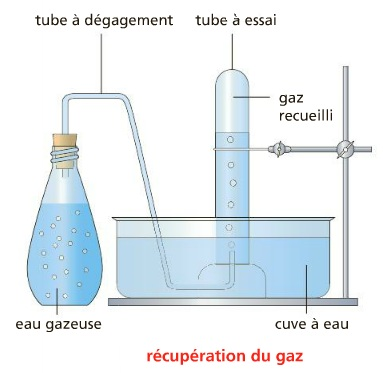
\includegraphics[scale=0.4]{recueilgaz}
		\end{column}

	
\end{columns}.
\end{mybilan}